%----------------------------------------------------------------------------------------
%    PACKAGES AND THEMES
%----------------------------------------------------------------------------------------

\documentclass[aspectratio=169,xcolor=dvipsnames]{beamer}
\usetheme{SimpleDarkBlue}

\usepackage{hyperref}
\usepackage{graphicx} % Allows including images
\usepackage{booktabs} % Allows the use of \toprule, \midrule and \bottomrule in tables

%----------------------------------------------------------------------------------------
%    TITLE PAGE
%----------------------------------------------------------------------------------------

\title{Traducción de lengua de signos basada en \textit{keypoints} con modelos pequeños del lenguaje}
%\subtitle{Subtitle}

\author{Nicolás Rodríguez Ruiz}

\institute
{
    Departamentp de Ciencias de la Computación e Inteligencia Artificial \\
    ESCUELA TÉCNICA SUPERIOR DE INGENIERIA INFORMÁTICA
}
\date{\today} % Date, can be changed to a custom date

%----------------------------------------------------------------------------------------
%    PRESENTATION SLIDES
%----------------------------------------------------------------------------------------

\begin{document}

\begin{frame}
    % Print the title page as the first slide
    \titlepage
\end{frame}

\begin{frame}{Overview}
    % Throughout your presentation, if you choose to use \section{} and \subsection{} commands, these will automatically be printed on this slide as an overview of your presentation
    \tableofcontents
\end{frame}

%------------------------------------------------
\section{Motivación y objetivos}
%------------------------------------------------

% --- Slide 1: Motivación / el reto de la comunicación ---
\begin{frame}{El reto de la comunicación}
    \begin{center}
        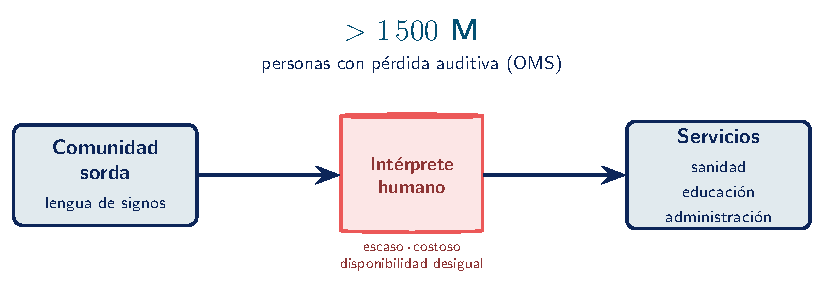
\includegraphics[width=0.92\linewidth]{images/intro/motivacion}
    \end{center}
    \begin{center}
        \small La lengua de signos es el medio natural de millones de personas,
        pero el acceso a servicios esenciales aún depende de un recurso escaso.
    \end{center}
\end{frame}

%------------------------------------------------

% --- Slide 2: Dos direcciones ---
\begin{frame}{Dos direcciones, un mismo objetivo: la inclusión}
    \begin{center}
        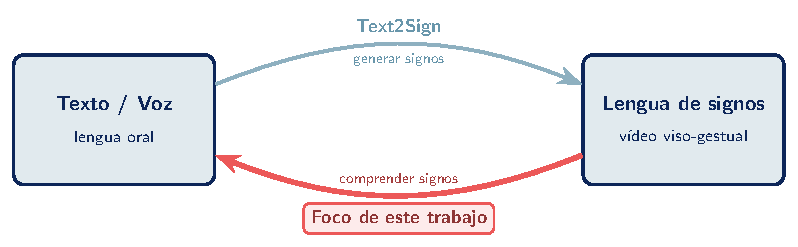
\includegraphics[width=0.85\linewidth]{images/intro/directions}
    \end{center}
    \begin{itemize}
        \item \textbf{Text2Sign}: generar signos para la comprensión de personas sordas.
        \item \alert{Sign2Text}: comprender los signos $\rightarrow$ \textbf{impacto directo en la autonomía comunicativa}.
    \end{itemize}
\end{frame}

%------------------------------------------------

% --- Slide 3: Sign2Text del vídeo al texto ---
\begin{frame}{Sign2Text: del vídeo al texto}
    \begin{center}
        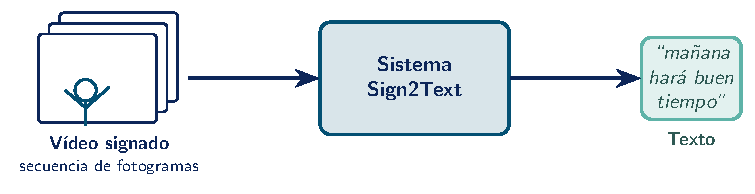
\includegraphics[width=0.9\linewidth]{images/intro/sign2text_pipeline}
    \end{center}
    \begin{block}{¿Qué habilita?}
        Subtitulado en tiempo real \quad·\quad asistentes que entienden a usuarios sordos
        \quad·\quad servicios públicos sin intérprete presente.
    \end{block}
\end{frame}

%------------------------------------------------

% --- Slide 4: Por qué es difícil (multimodalidad) ---
\begin{frame}{¿Por qué es difícil? Una señal multimodal}
    \begin{columns}[c]
        \column{0.6\textwidth}
        \begin{center}
            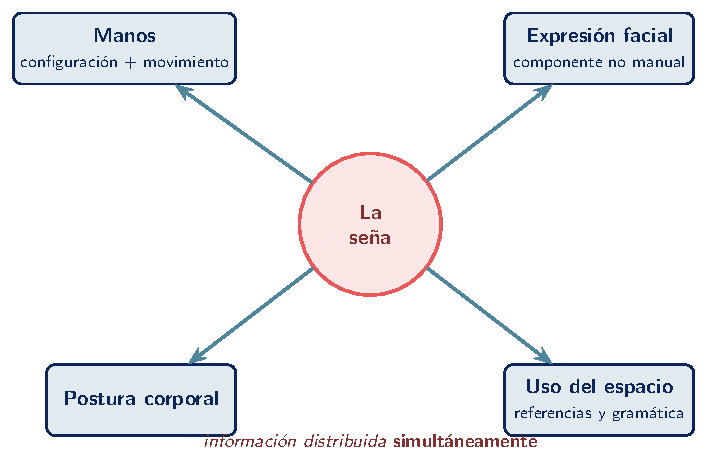
\includegraphics[width=\linewidth]{images/intro/multimodal}
        \end{center}
        \column{0.4\textwidth}
        \footnotesize
        A diferencia del habla (señal 1D), la información se distribuye en varios canales a la vez.
        \begin{itemize}
            \item Gran \textbf{variedad} de lenguas de signos.
            \item Normalmente \textbf{sin relación gramatical} con la lengua oral de la región.
        \end{itemize}
    \end{columns}
\end{frame}

%------------------------------------------------

% --- Slide 5: Keypoints ---
\begin{frame}{Keypoints: privacidad y eficiencia}
    \begin{center}
        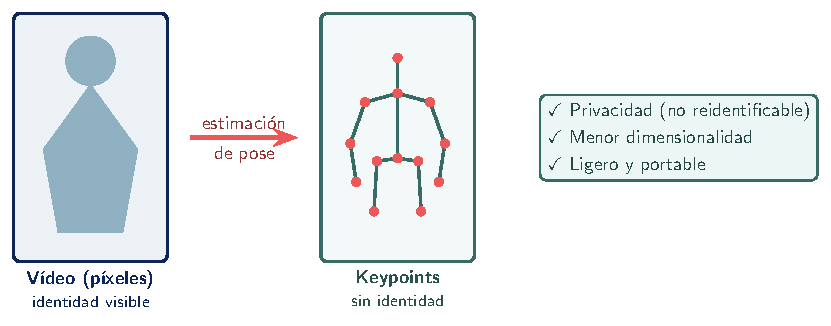
\includegraphics[width=0.95\linewidth]{images/intro/keypoints}
    \end{center}
    \begin{center}
        \small Puntos predefinidos del cuerpo que capturan el gesto
        \alert{sin preservar la identidad visual} y reducen drásticamente la dimensionalidad.
    \end{center}
\end{frame}

%------------------------------------------------

% --- Slide 6: Objetivo principal ---
\begin{frame}{Objetivo principal}
    \begin{block}{Meta}
        Demostrar la viabilidad de un sistema \textbf{Sign2Text} basado en representaciones
        intermedias (\textbf{glosas} y \textbf{keypoints}) mediante un
        \alert{Modelo Pequeño de Lenguaje} \textit{decoder-only}, manteniendo
        \textbf{ejecución local} y \textbf{privacidad}.
    \end{block}
    \begin{center}
        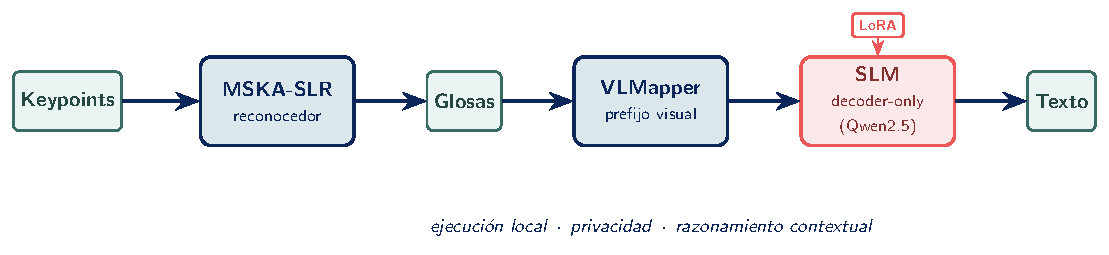
\includegraphics[width=0.95\linewidth]{images/intro/objetivo_pipeline}
    \end{center}
\end{frame}

%------------------------------------------------

% --- Slide 7: Objetivos específicos ---
\begin{frame}{Objetivos específicos}
    \begin{center}
        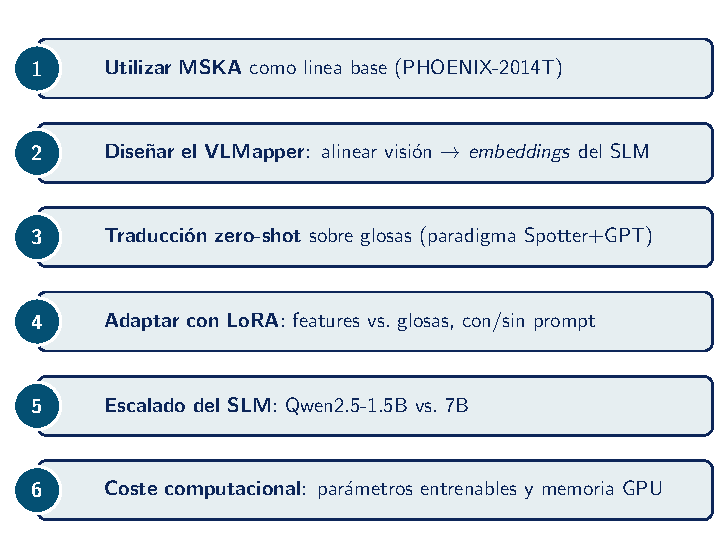
\includegraphics[height=0.82\textheight]{images/intro/objetivos}
    \end{center}
\end{frame}


%------------------------------------------------
\section{Estado del arte}
%------------------------------------------------

% --- Slide 1: evolución ---
\begin{frame}{Una evolución de arquitecturas}
    \begin{center}
        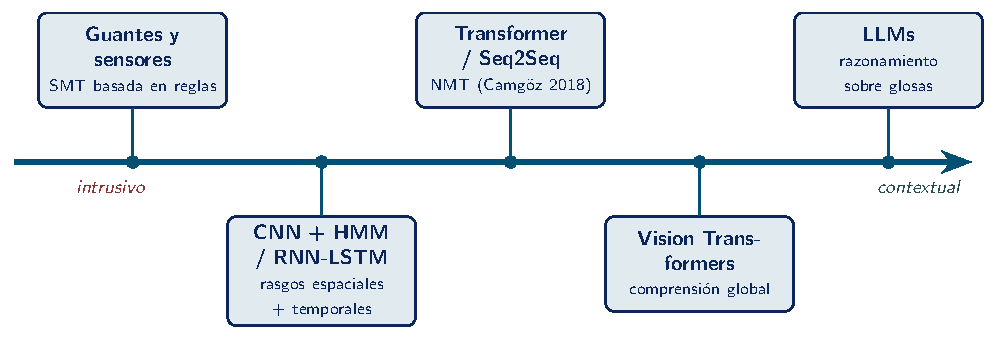
\includegraphics[width=\linewidth]{images/sota/sota_timeline}
    \end{center}
    \begin{center}
        \small Del \textit{hardware} intrusivo y las reglas manuales
        al razonamiento contextual; el reconocimiento pasa de \textbf{aislado} a
        \textbf{continuo}, más cercano a la comunicación real.
    \end{center}
\end{frame}

%------------------------------------------------

% --- Slide 2: con glosas vs sin glosas ---
\begin{frame}{Con glosas frente a sin glosas}
    \begin{center}
        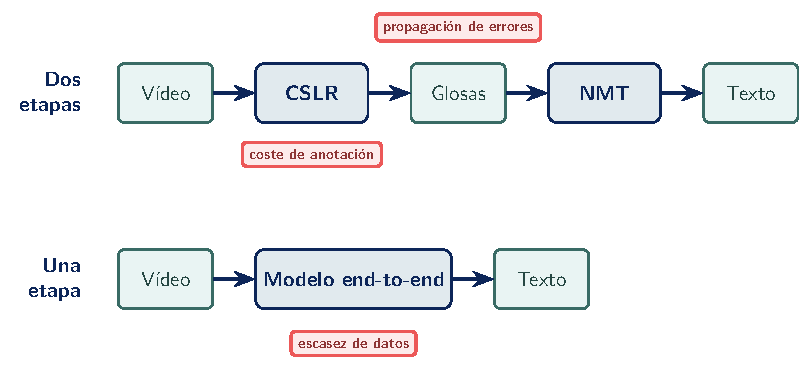
\includegraphics[width=0.85\linewidth]{images/sota/sota_paradigms}
    \end{center}
    \begin{itemize}
        \item \textbf{Dos etapas}: las glosas dan estructura, pero \alert{propagan errores} y exigen anotación experta.
        \item \textbf{Una etapa}: elimina el cuello de botella, pero se \alert{estanca} por la escasez de datos.
    \end{itemize}
\end{frame}

%------------------------------------------------

% --- Slide 3: renacer de las glosas con LLMs ---
\begin{frame}{El renacer de las glosas con LLMs: Spotter+GPT}
    \begin{center}
        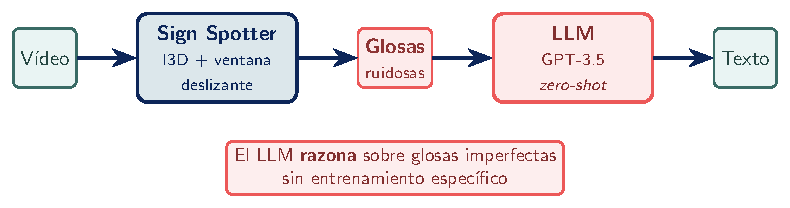
\includegraphics[width=0.9\linewidth]{images/sota/sota_spottergpt}
    \end{center}
    \begin{columns}[T]
        \column{0.5\textwidth}
        \begin{block}{LLM}
            El LLM tolera glosas ruidosas \emph{zero-shot}: BLEURT $46.9$ vs.\ $19.9$ del \textit{transformer}.
        \end{block}
        \column{0.5\textwidth}
        \begin{alertblock}{Límites para el despliegue}
            Nube, coste de API, \textbf{privacidad} y latencia $\rightarrow$ inviable en tiempo real y local.
        \end{alertblock}
    \end{columns}
\end{frame}

%------------------------------------------------

% --- Slide 4: keypoints y MSKA ---
\begin{frame}{Keypoints y MSKA: el hueco que motiva el SLM}
    \begin{center}
        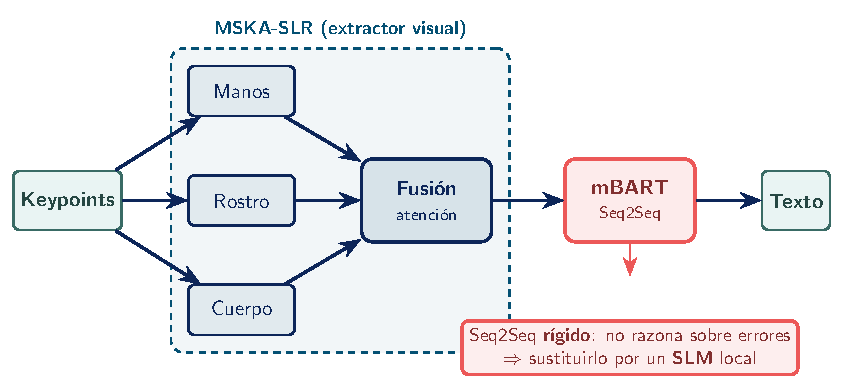
\includegraphics[width=0.85\linewidth]{images/sota/sota_mska}
    \end{center}
    \begin{center}
        \small MSKA desacopla manos, rostro y cuerpo en flujos de atención,
        pero lo acopla a un decodificador \textbf{mBART} rígido: aquí entra nuestro
        \alert{Modelo Pequeño de Lenguaje}.
    \end{center}
\end{frame}

%------------------------------------------------

% --- Slide 5: datasets ---
\begin{frame}{Conjuntos de datos: por qué PHOENIX-2014T}
    \begin{table}
        \small
        \begin{tabular}{lllcc}
            \toprule
            \textbf{Corpus} & \textbf{Lengua} & \textbf{Dominio} & \textbf{Keypoints} & \textbf{Acceso} \\
            \midrule
            \alert{PHOENIX-2014T} & DGS (alemán) & Meteorología & No & Público \\
            CSL-Daily             & CSL (chino)  & Cotidiano    & No & Restringido \\
            How2Sign              & ASL (inglés) & Instructivo  & Sí (2D) & Público \\
            LSE-eSaude            & LSE (español)& Salud        & No & Público \\
            \bottomrule
        \end{tabular}
    \end{table}
    \vspace{0.4em}
    \begin{block}{Elección}
        \textbf{Estándar de oro} (comparabilidad con casi una década de literatura),
        \textbf{corpus original de MSKA} (base de referencia exacta) y \textbf{acceso público}
        (reproducibilidad).
    \end{block}
\end{frame}

%------------------------------------------------
\section{Fundamentos}
%------------------------------------------------

% --- Slide 1: métricas ---
\begin{frame}{Métricas: de lo léxico a lo semántico}
    \begin{center}
        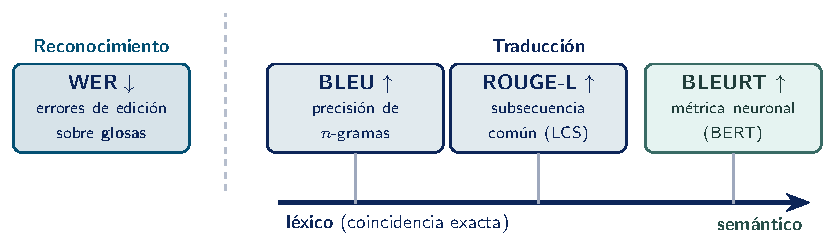
\includegraphics[width=\linewidth]{images/fundamentos/metricas}
    \end{center}
    \begin{itemize}
        \item \textbf{WER} mide el error sobre las \textbf{glosas} (reconocimiento).
        \item BLEU y ROUGE-L comparan \textbf{coincidencia léxica}; \alert{BLEURT} valora el \textbf{significado} (sinónimos y paráfrasis).
    \end{itemize}
\end{frame}

%------------------------------------------------

% --- Slide 2: Transformer / decoder-only ---
\begin{frame}{Transformer y modelos \textit{decoder-only}}
% %     \begin{center}
% %         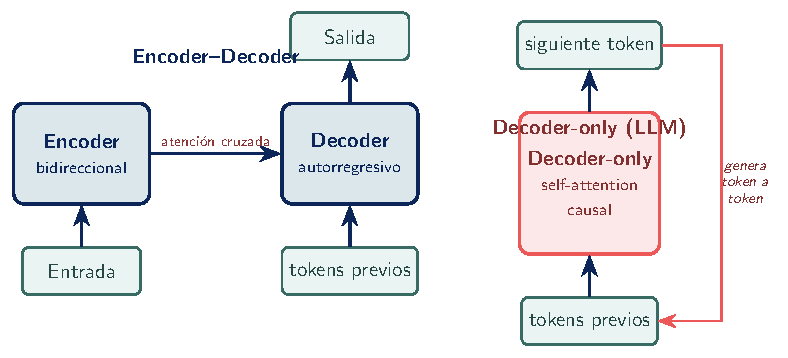
\includegraphics[width=0.92\linewidth]{images/fundamentos/decoder_only}
% %     \end{center}
%     \begin{center}
%         \small La \textbf{autoatención} relaciona cada elemento con todos en paralelo.
%         Un LLM \alert{decoder-only} prescinde del codificador y genera texto de forma
%         autorregresiva; su escalado produce \textbf{capacidades emergentes} (\textit{zero-shot}).
%     \end{center}
\end{frame}

%------------------------------------------------

% --- Slide 3: LoRA ---
\begin{frame}{Adaptación eficiente: LoRA}
    \begin{center}
        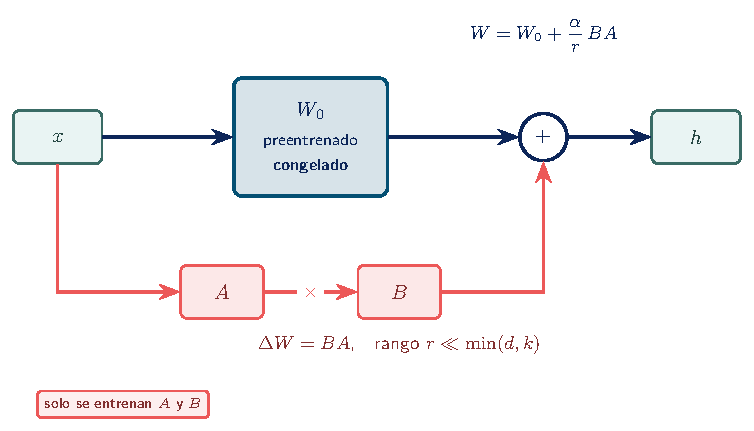
\includegraphics[width=0.9\linewidth]{images/fundamentos/lora}
    \end{center}
    \begin{center}
        \small Se \textbf{congelan} los pesos preentrenados y solo se entrena una
        actualización de \alert{rango bajo} $\Delta W = BA$. Adaptar el modelo con una
        fracción mínima de parámetros hace viable el \textit{finetuning} local.
    \end{center}
\end{frame}

%------------------------------------------------

% --- Slide 4: CTC ---
\begin{frame}{El esqueleto como dato: alineación con CTC}
    \begin{center}
        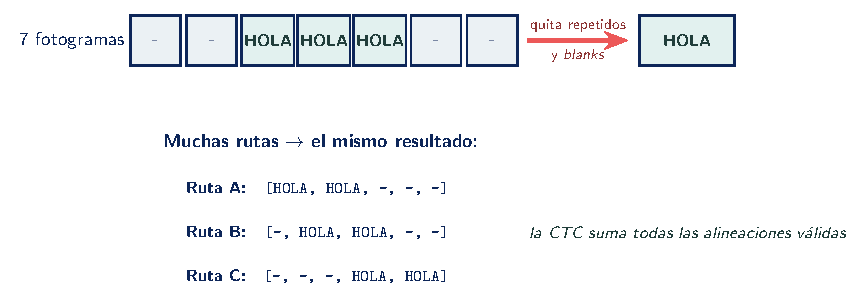
\includegraphics[width=0.92\linewidth]{images/fundamentos/ctc}
    \end{center}
    \begin{center}
        \small La secuencia de \textit{keypoints} es mucho más larga que la de glosas y no
        está segmentada. \alert{CTC} alinea ambas sumando todas las rutas válidas, sin
        anotar el instante exacto de cada signo.
    \end{center}
\end{frame}

%------------------------------------------------

% --- Slide 5: DSTA intuición ---
\begin{frame}{DSTA: atención espacio-temporal desacoplada}
    \begin{center}
        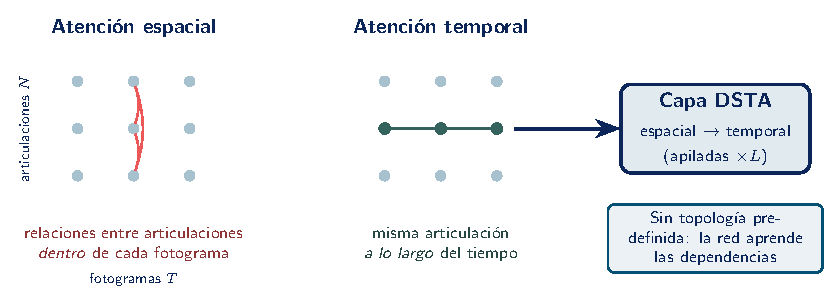
\includegraphics[width=\linewidth]{images/fundamentos/dsta}
    \end{center}
    \begin{center}
        \small Separar el modelado \textbf{espacial} (entre articulaciones) del
        \textbf{temporal} (a lo largo del tiempo) abarata el cómputo y respeta la
        estructura del esqueleto. Es el bloque base de \alert{MSKA}.
    \end{center}
\end{frame}

%------------------------------------------------

% --- Slide 6: DSTA estrategias de desacoplamiento ---
\begin{frame}{DSTA: tres estrategias de desacoplamiento}
    \begin{center}
        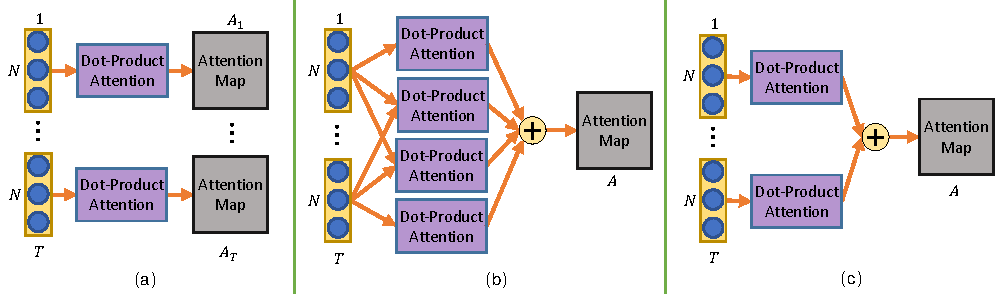
\includegraphics[width=0.95\linewidth]{images/DSTA/strategy}
    \end{center}
    \begin{itemize}
        \footnotesize
        \item \textbf{(a)} un mapa por fotograma: sin contexto global.
        \item \textbf{(b)} un mapa entre todos los fotogramas: potente pero \alert{muy costoso}.
        \item \alert{(c)} suma los mapas por fotograma $\rightarrow$ un \textbf{único producto} $N\!\times\!N$: mismo resultado, mucho más eficiente.
    \end{itemize}
\end{frame}

%------------------------------------------------

% --- Slide 7: DSTA codificación posicional ---
\begin{frame}{DSTA: codificación posicional espacial y temporal}
    \begin{columns}[T]
        \column{0.5\textwidth}
        \begin{center}
            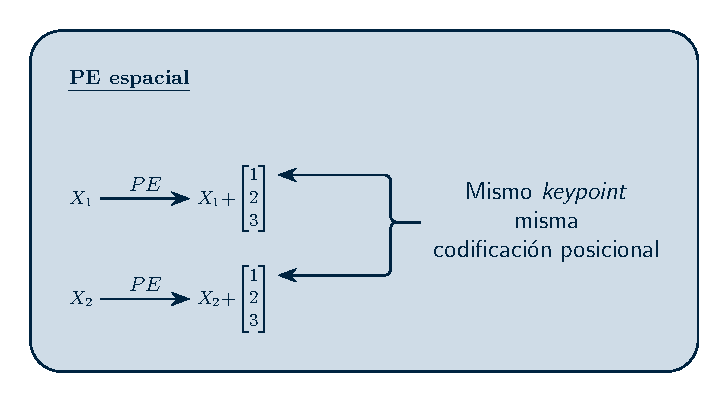
\includegraphics[width=0.92\linewidth]{images/DSTA/DSTA-SPE}\\[2pt]
            \footnotesize \textbf{Espacial}: la misma articulación conserva su identidad en todo fotograma.
        \end{center}
        \column{0.5\textwidth}
        \begin{center}
            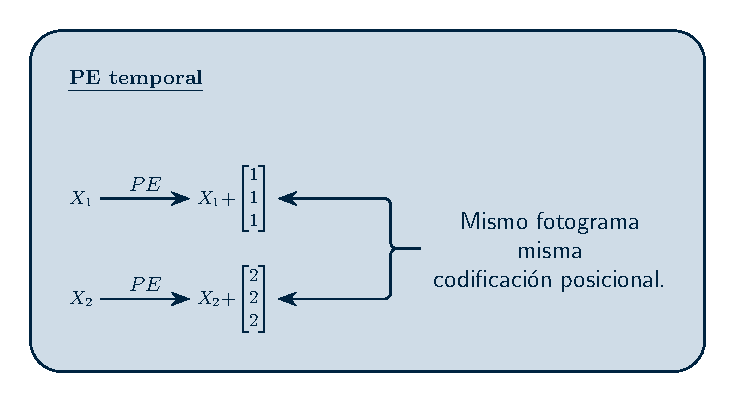
\includegraphics[width=0.92\linewidth]{images/DSTA/DSTA-TPE}\\[2pt]
            \footnotesize \textbf{Temporal}: se codifica el instante; dentro del fotograma no varía.
        \end{center}
    \end{columns}
    \vspace{0.3em}
    \begin{center}
        \small Una PE ingenua sobre el tensor aplanado daría a la misma articulación
        códigos dispares en distintos fotogramas; \alert{separar espacio y tiempo} preserva la semántica del esqueleto.
    \end{center}
\end{frame}

%------------------------------------------------

% --- Slide 8: DSTA módulo de atención espacial ---
\begin{frame}{DSTA: el módulo de atención espacial}
    \begin{center}
        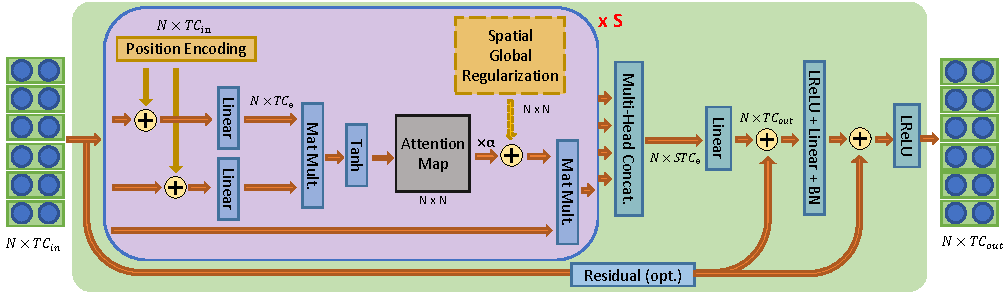
\includegraphics[width=\linewidth]{images/DSTA/attention}
    \end{center}
    \begin{itemize}
        \footnotesize
        \item \textbf{SGR}: mapa global entrenable $N\!\times\!N$ que aporta la anatomía (constante entre sujetos), solo en la dimensión espacial.
        \item \alert{Tanh} en lugar de \textit{softmax}: permite relaciones \textbf{negativas} entre articulaciones. $S$ cabezas y conexiones residuales.
    \end{itemize}
\end{frame}

%------------------------------------------------

% --- Slide 9: DSTA-Net pipeline ---
\begin{frame}{DSTA-Net: la estructura completa}
    \begin{center}
        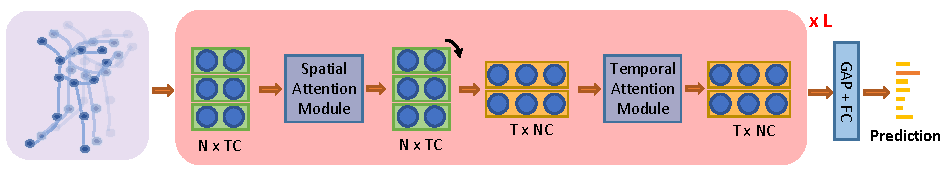
\includegraphics[width=\linewidth]{images/DSTA/pipeline}
    \end{center}
    \begin{center}
        \small Cada una de las $L$ capas encadena \textbf{atención espacial} $\rightarrow$ \textbf{transposición}
        $\rightarrow$ \textbf{atención temporal}. Es el bloque que MSKA adapta por cada flujo de \textit{keypoints}.
    \end{center}
\end{frame}

%------------------------------------------------
\section{Metodología}
%------------------------------------------------

% --- Slide 1: visión general del pipeline ---
\begin{frame}{Visión general del sistema}
    \begin{center}
        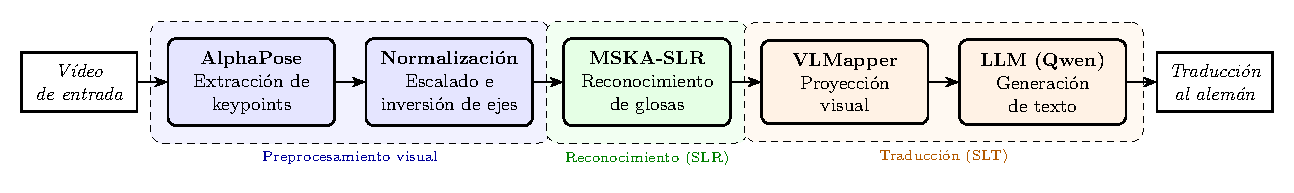
\includegraphics[width=\linewidth]{images/MSKA/pipeline_overview}
    \end{center}
    \begin{center}
        \small Un flujo de \textbf{tres etapas}: extracción de \textit{keypoints}
        (AlphaPose), reconocimiento de \textbf{glosas} (MSKA-SLR) y \textbf{traducción}
        (VLMapper $+$ SLM). Las secciones siguen este orden.
    \end{center}
\end{frame}

%------------------------------------------------

% --- Slide 2: elección de herramienta de pose ---
\begin{frame}{Extracción de \textit{keypoints}: ¿qué herramienta?}
    \begin{center}
        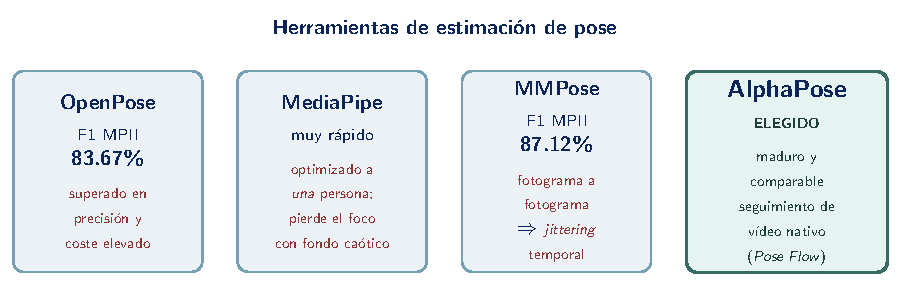
\includegraphics[width=\linewidth]{images/metodologia/tools}
    \end{center}
    \begin{center}
        \small El dominio exige \textbf{coherencia temporal} y robustez con varias personas
        en escena. Elegimos \alert{AlphaPose}: maduro, comparable con la literatura y con
        \textbf{seguimiento de vídeo nativo}.
    \end{center}
\end{frame}

%------------------------------------------------

% --- Slide 3: AlphaPose top-down y robustez ---
\begin{frame}{AlphaPose: enfoque \textit{top-down} y robustez}
    \begin{center}
        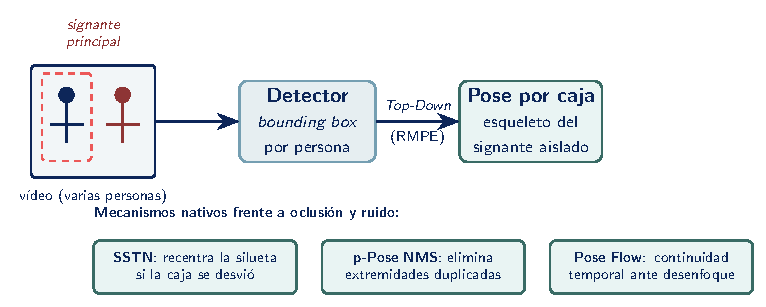
\includegraphics[width=0.95\linewidth]{images/metodologia/alphapose}
    \end{center}
    \begin{center}
        \small La estrategia \textbf{descendente} (RMPE) detecta primero a cada persona y
        luego estima su pose, \alert{blindando al signante} frente al ruido del entorno.
    \end{center}
\end{frame}

%------------------------------------------------

% --- Slide 4: jittering y HALPE-136 ---
\begin{frame}{El dilema del \textit{jittering}: no suavizar}
    \begin{center}
        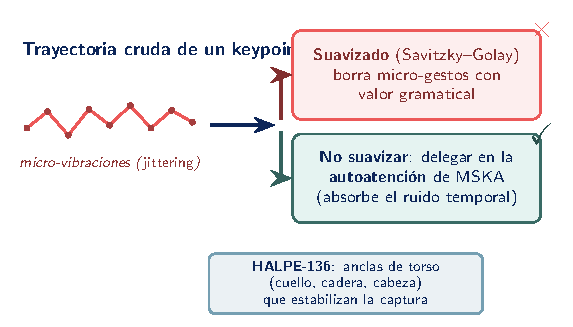
\includegraphics[width=0.95\linewidth]{images/metodologia/jitter}
    \end{center}
    \begin{center}
        \small Un suavizado estadístico podría \alert{borrar micro-gestos con valor gramatical}.
        Preferimos delegar el ruido temporal en la \textbf{autoatención} de la red.
    \end{center}
\end{frame}

%------------------------------------------------

% --- Slide 5: normalización ---
\begin{frame}{Normalización de los datos espaciales}
    \begin{center}
        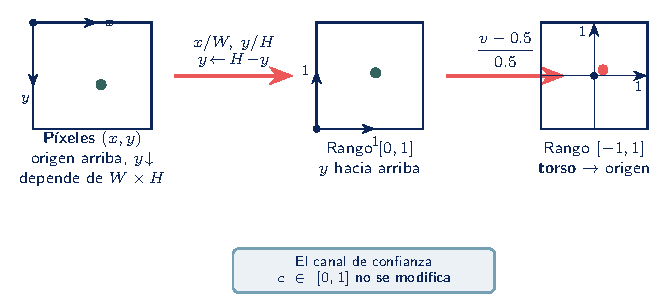
\includegraphics[width=\linewidth]{images/metodologia/normalizacion}
    \end{center}
    \begin{center}
        \small Independencia de la resolución y estabilidad numérica: se lleva todo al rango
        \textbf{$[-1,1]$} con el \textbf{torso} (referencia global) mapeado al origen.
    \end{center}
\end{frame}

%------------------------------------------------

% --- Slide 6: aumento de datos ---
\begin{frame}{Aumento de datos: combatir la escasez}
    \begin{center}
        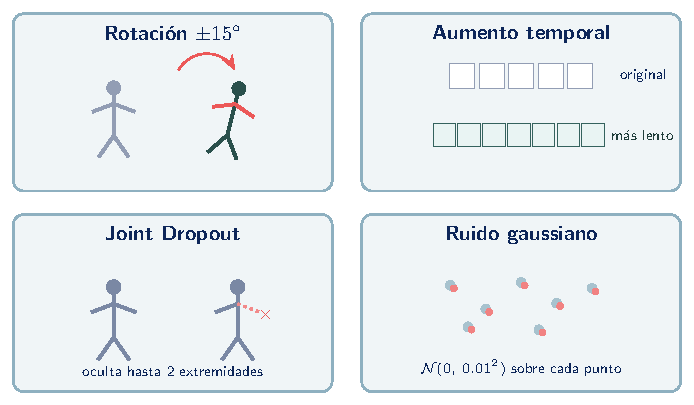
\includegraphics[width=0.92\linewidth]{images/metodologia/augmentation}
    \end{center}
    \begin{center}
        \small Con $\sim$7000 vídeos, la regularización es clave. Solo se conservan
        \textbf{rotaciones} (las traslaciones y el \textit{zoom} degradaban), sumando
        \textit{Joint Dropout} y \textbf{ruido gaussiano}.
    \end{center}
\end{frame}

%------------------------------------------------

% --- Slide 7: MSKA-SLR arquitectura ---
\begin{frame}{MSKA-SLR: cuatro flujos desacoplados}
    \begin{center}
        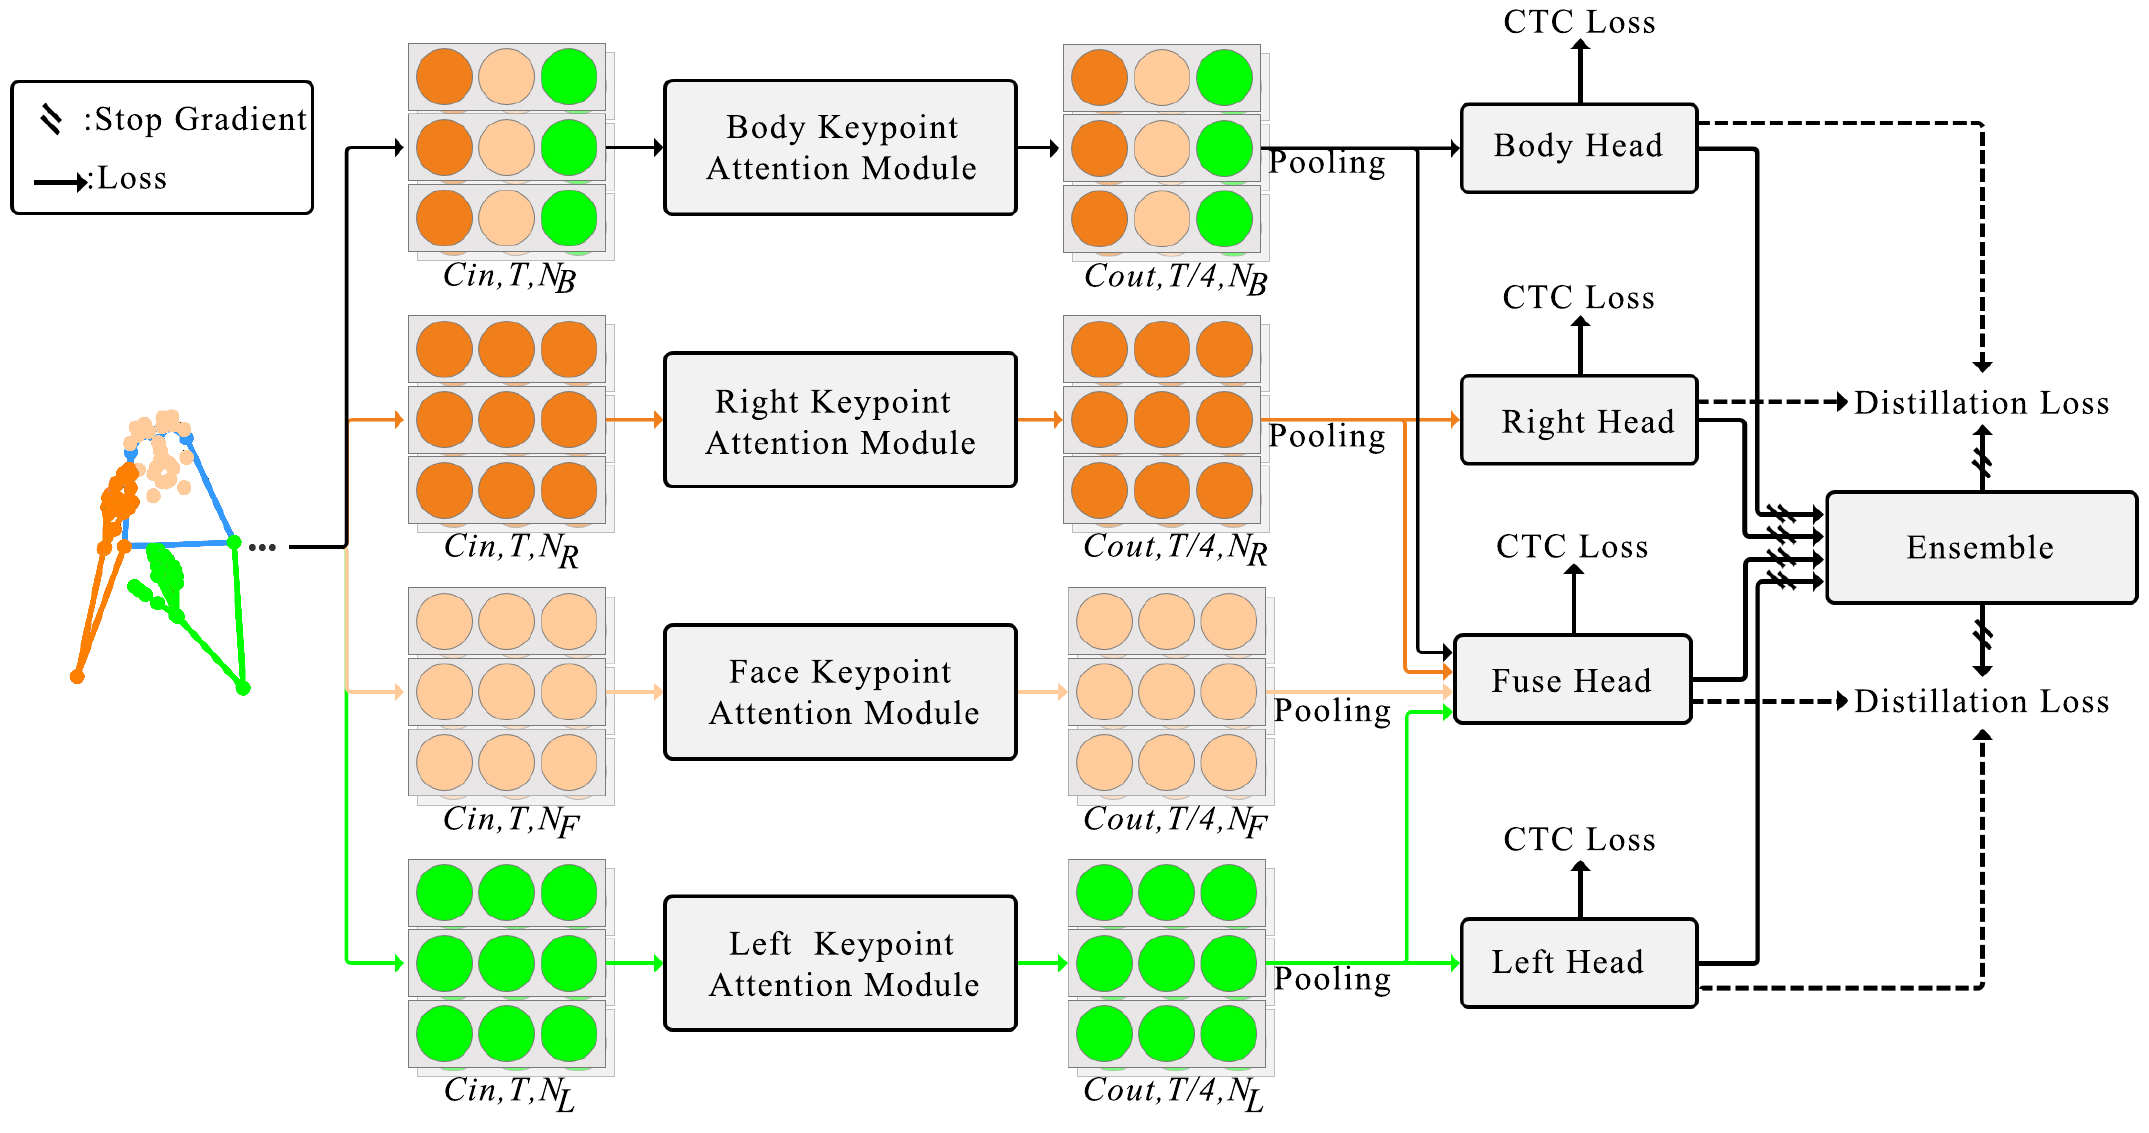
\includegraphics[width=0.98\linewidth]{images/MSKA/MSKA_SLR}
    \end{center}
    \begin{center}
        \small Manos, rostro y cuerpo se procesan por separado para que los \textbf{detalles finos}
        no se pierdan. El \textbf{rostro} aporta contexto a las manos y a la fusión,
        \alert{sin cabeza de clasificación propia}.
    \end{center}
\end{frame}

%------------------------------------------------

% --- Slide 8: módulo de atención de keypoints ---
\begin{frame}{Dentro del flujo: módulo de atención de \textit{keypoints}}
    \begin{center}
        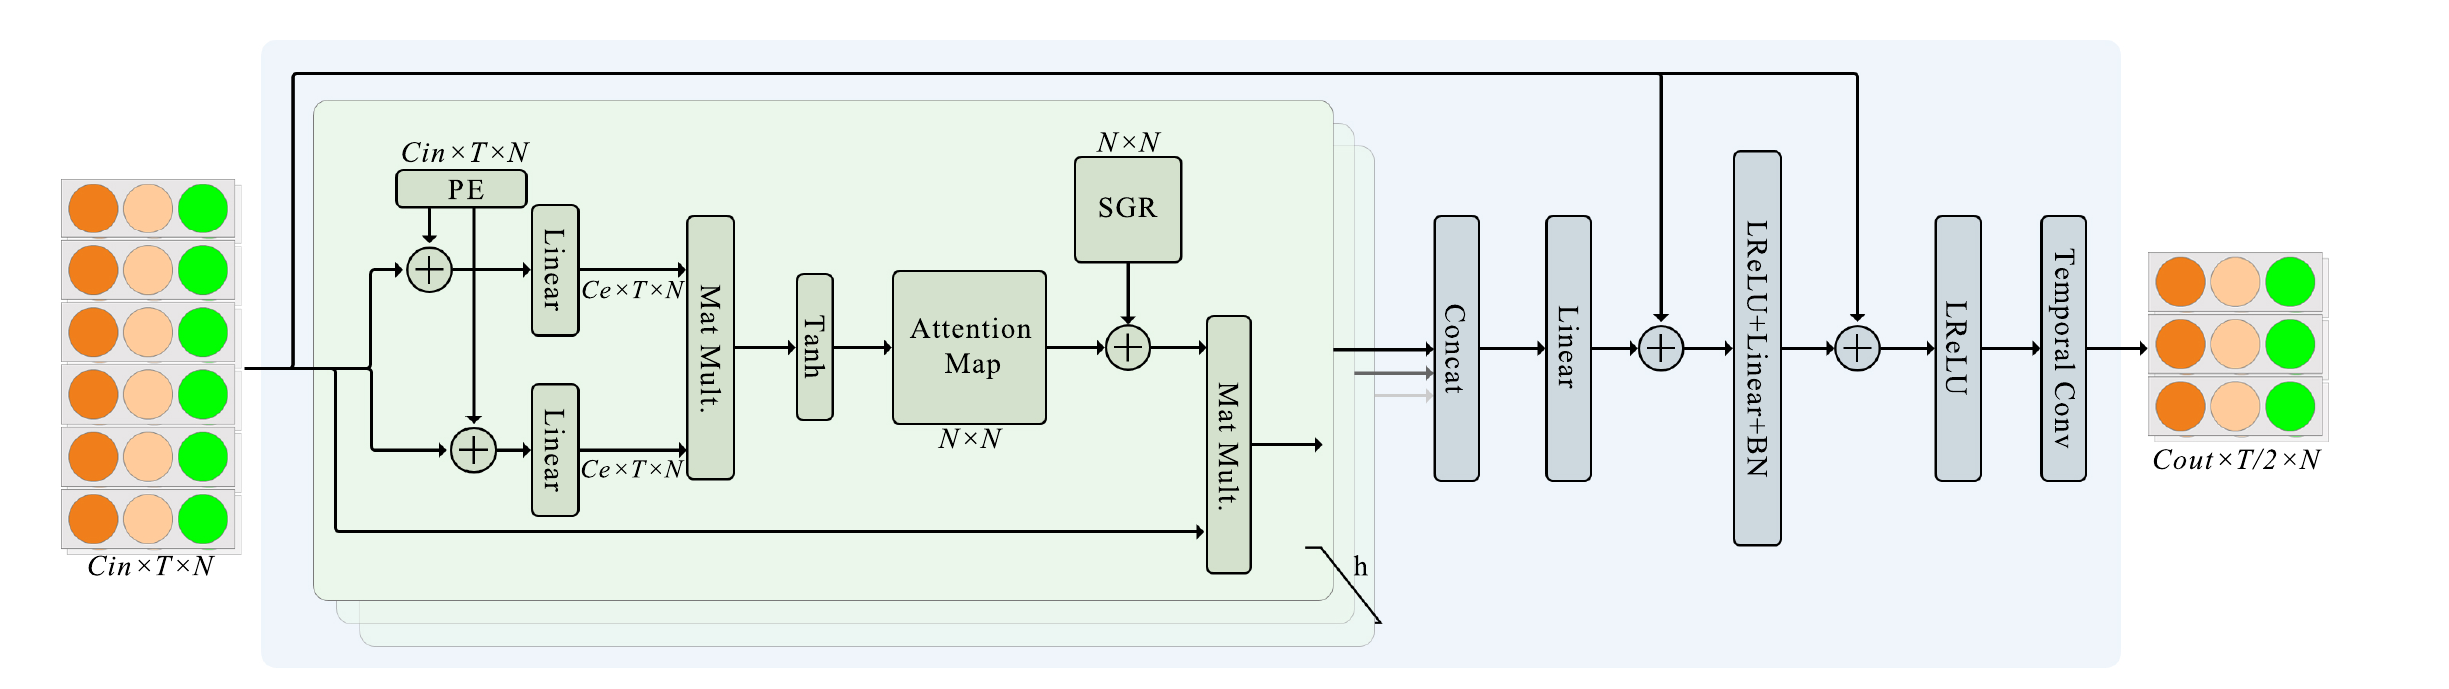
\includegraphics[width=\linewidth]{images/MSKA/MSKA_att}
    \end{center}
    \begin{itemize}
        \item Codificación posicional \textbf{solo espacial}; el tiempo se modela con
        \textbf{convoluciones 2D} $\rightarrow$ menos parámetros, menos sobreajuste.
        \item Cascada de \textbf{8 bloques} que contrae $T\!\rightarrow\!T/4$ y expande los canales hasta $256$.
    \end{itemize}
\end{frame}

%------------------------------------------------

% --- Slide 8b: redes de cabecera ---
\begin{frame}{Redes de cabecera y fusión}
    \begin{center}
        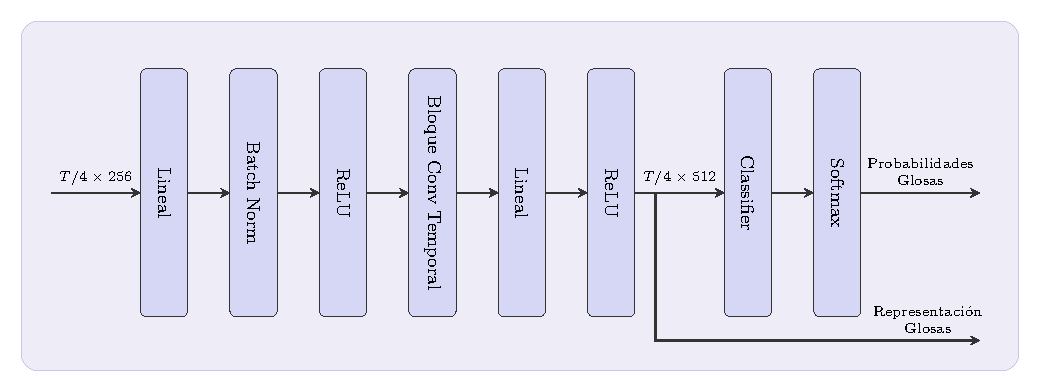
\includegraphics[width=\linewidth]{images/MSKA/headNet}
    \end{center}
    \begin{center}
        \small Cada flujo tiene su cabecera (produce la \textbf{representación de glosa}, $T/4\times512$),
        y un \alert{Cabezal de Fusión} integra los cuatro. En inferencia sus probabilidades se
        promedian en un \textit{ensemble}.
    \end{center}
\end{frame}

%------------------------------------------------

% --- Slide 9: pérdida y autodestilación ---
\begin{frame}{Pérdida: CTC más autodestilación}
    \begin{columns}[c]
        \column{0.62\textwidth}
        \begin{center}
            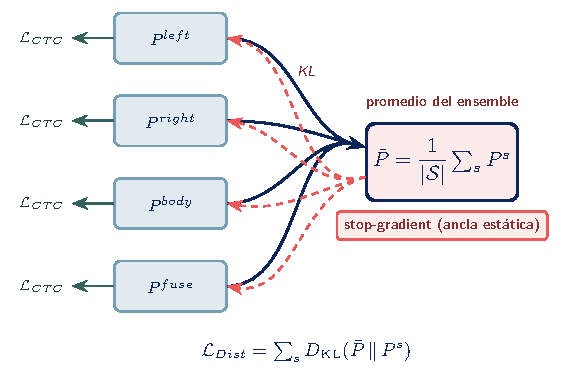
\includegraphics[width=\linewidth]{images/metodologia/distill}
        \end{center}
        \column{0.38\textwidth}
        \footnotesize
        Cada cabeza se supervisa con \textbf{CTC}. Además, el promedio del \textit{ensemble}
        actúa como \alert{pseudo-objetivo}: la divergencia \textbf{KL} acerca cada flujo al
        conocimiento global.
        \vspace{0.4em}
        \begin{block}{\textit{Stop-gradient}}
            El promedio es un \textbf{ancla estática}; evita el colapso del modelo.
        \end{block}
    \end{columns}
\end{frame}

%------------------------------------------------

% --- Slide 10: de mBART al SLM (contribución clave) ---
\begin{frame}{Del reconocimiento a la traducción: de mBART al SLM}
    \begin{center}
        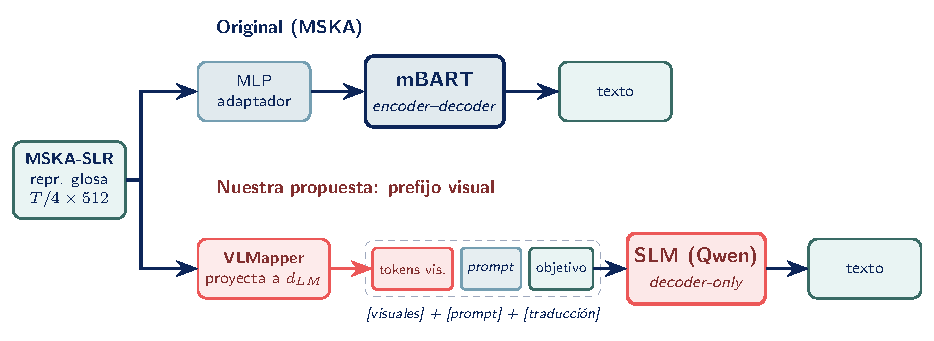
\includegraphics[width=\linewidth]{images/metodologia/mbart_vs_slm}
    \end{center}
    \begin{center}
        \small En lugar del \textbf{mBART} rígido, proyectamos la representación de glosa con el
        \alert{VLMapper} y la anteponemos como \textbf{prefijo visual} a un SLM
        \textit{decoder-only}, aprovechando su razonamiento contextual.
    \end{center}
\end{frame}

%------------------------------------------------

% --- Slide 11: VLMapper, LoRA y zero-shot ---
\begin{frame}{Adaptación eficiente: VLMapper, LoRA y \textit{zero-shot}}
    \begin{columns}[c]
        \column{0.6\textwidth}
        \begin{center}
            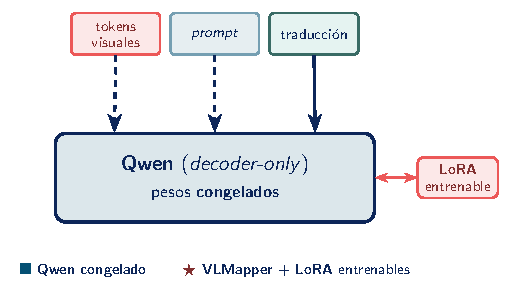
\includegraphics[width=\linewidth]{images/metodologia/train}
        \end{center}
        \column{0.4\textwidth}
        \footnotesize
        La pérdida se aplica \textbf{solo sobre la traducción}. Se congela Qwen y se entrenan
        el \alert{VLMapper} ($\approx$0.5--1.8\,M par.) y los adaptadores \textbf{LoRA}.
        \begin{alertblock}{\textit{Zero-shot}}
            Como \textbf{Spotter+GPT}: pasar las glosas como texto a Qwen2.5-14B sin entrenar,
            como línea base.
        \end{alertblock}
    \end{columns}
\end{frame}

%------------------------------------------------
\section{Experimentación y resultados}
%------------------------------------------------

% --- Slide 1: configuración experimental ---
\begin{frame}{Configuración experimental}
    \begin{columns}[T]
        \column{0.5\textwidth}
        \begin{block}{Entorno}
            \footnotesize
            \begin{itemize}
                \item 1$\times$ \textbf{NVIDIA A100} (40\,GB), \texttt{bfloat16}.
                \item PyTorch $+$ \textit{Transformers} (Hugging Face).
                \item Optimizador \textbf{AdamW}, \textit{cosine decay}, \textit{early stopping}.
            \end{itemize}
        \end{block}
        \column{0.5\textwidth}
        \begin{block}{LoRA}
            \footnotesize
            \begin{itemize}
                \item Rango $r=64$, $\alpha=128$ $\Rightarrow$ escala $\alpha/r=2$, \textit{dropout} $0.25$.
                \item \textbf{LoRA-Att}: solo atención. \quad \textbf{LoRA-All}: $+$ FFN.
                \item Qwen congelado; \textit{Full} solo viable en 1.5B.
            \end{itemize}
        \end{block}
    \end{columns}
    \vspace{0.3em}
    \begin{center}
        \small Evaluación sobre \textbf{PHOENIX-2014T}: reconocimiento con \textbf{WER}
        y traducción con \textbf{BLEU} y \textbf{ROUGE-L} (más \textbf{BLEURT} en \textit{zero-shot}).
    \end{center}
\end{frame}

%------------------------------------------------

% --- Slide 2: dataset ---
\begin{frame}{El corpus PHOENIX-2014T de un vistazo}
    \begin{center}
        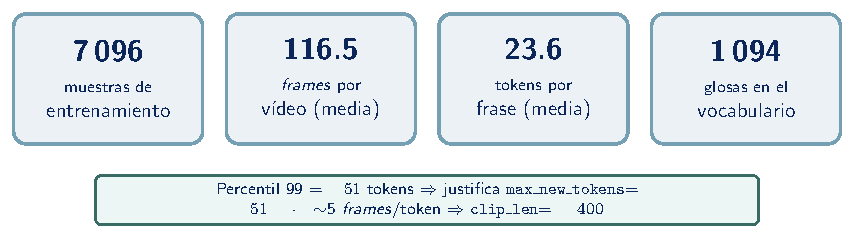
\includegraphics[width=\linewidth]{images/experimentacion/dataset}
    \end{center}
    \begin{center}
        \small Corpus \textbf{pequeño} y de dominio acotado (meteorología): la escasez de datos
        será el hilo conductor del análisis.
    \end{center}
\end{frame}

%------------------------------------------------

% --- Slide 3: SLR aumento de datos ---
\begin{frame}{Reconocimiento (SLR): estudio de aumento de datos}
    \begin{table}
        \small
        \begin{tabular}{lccccc}
            \toprule
            \textbf{Configuración} & \textbf{Dev WER}$\downarrow$ & \textbf{Test WER}$\downarrow$ & \textbf{SUB} & \textbf{DEL} & \textbf{INS} \\
            \midrule
            SLR-base                 & 27.81 & 27.33 & 11.81 & 13.29 & 2.23 \\
            \alert{SLR-JointDropout} & \textbf{27.68} & \textbf{27.24} & 12.28 & 12.51 & 2.44 \\
            SLR-StructuredDropout    & 28.24 & 27.59 & 12.82 & 12.21 & 2.56 \\
            SLR-GaussianNoise        & 28.56 & 28.13 & 12.82 & 13.15 & 2.16 \\
            \bottomrule
        \end{tabular}
    \end{table}
    \vspace{0.3em}
    \begin{center}
        \small El aumento apenas ayuda ($<0.1$ pts de WER). \alert{Joint Dropout}, la variante
        más suave, gana por poco: reduce \textbf{eliminaciones} a costa de más sustituciones.
    \end{center}
\end{frame}

%------------------------------------------------

% --- Slide 4: SLR curvas + cualitativo ---
\begin{frame}{SLR: sobreajuste y análisis cualitativo}
    \begin{center}
        
\includegraphics[width=0.9\linewidth]{images/SLR/SLR_hr}
    \end{center}
    \begin{center}
        \footnotesize Brecha persistente entrenamiento ($\sim$15) vs.\ validación ($\sim$45): el
        \alert{corpus reducido} es la limitación, no la regularización. Errores como
        \textit{AUFLOESEN}$\rightarrow$\textit{VERSCHWINDEN} (sinónimos) \textbf{motivan un LLM} en la traducción.
    \end{center}
\end{frame}

%------------------------------------------------

% --- Slide 5: mBART línea base ---
\begin{frame}{Traducción: la línea base mBART}
    \begin{center}
        \begin{tabular}{lcccccc}
            \toprule
            \textbf{Modelo} & \textbf{B1} & \textbf{B2} & \textbf{B3} & \textbf{B4} & \textbf{ROUGE-L} \\
            \midrule
            MSKA-mBART (test) & 45.03 & 34.51 & 27.43 & \textbf{22.48} & \textbf{45.00} \\
            \bottomrule
        \end{tabular}
    \end{center}
    \vspace{0.4em}
    \begin{block}{Referencia sólida}
        BLEU-4 de \textbf{22.48} coherente con la literatura (valida nuestra reimplementación).
        Su arquitectura \textit{encoder-decoder} con \textbf{preentrenamiento multilingüe} en alemán
        generaliza bien: Dev y Test casi idénticos.
    \end{block}
\end{frame}

%------------------------------------------------

% --- Slide 6: zero-shot ---
\begin{frame}{Traducción \textit{zero-shot}: Spotter + Qwen-14B}
    \begin{center}
        \small BLEU-4 $=0.46$ \quad·\quad ROUGE-L $=9.85$ \quad·\quad \textbf{BLEURT} $=0.50$
        (vs.\ $0.49$ de Spotter+GPT con glosas ruidosas).
    \end{center}
    \begin{columns}[T]
        \column{0.33\textwidth}
        \begin{alertblock}{Escasez de glosas}
            \footnotesize Secuencias cortas $\rightarrow$ responde \textit{``Keine Übersetzung''}.
        \end{alertblock}
        \column{0.33\textwidth}
        \begin{alertblock}{Rompe la instrucción}
            \footnotesize Añade comentarios en lugar de traducir.
        \end{alertblock}
        \column{0.33\textwidth}
        \begin{alertblock}{Alucinación multilingüe}
            \footnotesize Genera texto en \textbf{chino} a mitad de la respuesta.
        \end{alertblock}
    \end{columns}
    \begin{center}
        \small La brecha con mBART justifica el \alert{\textit{finetuning}}.
    \end{center}
\end{frame}

%------------------------------------------------

% --- Slide 7: ablación modalidad y LoRA ---
\begin{frame}{Ablación (Qwen-1.5B): modalidad de entrada y LoRA}
    \begin{columns}[c]
        \column{0.6\textwidth}
        \begin{center}
            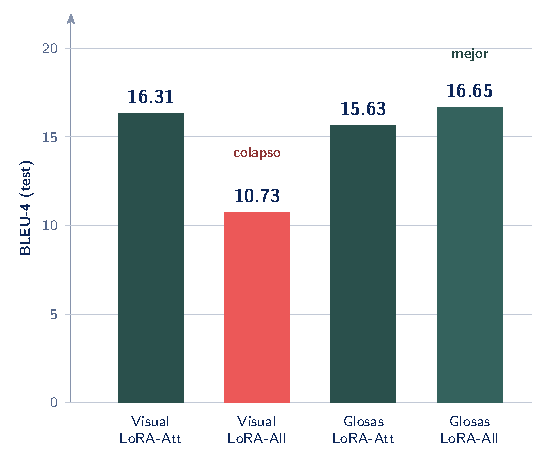
\includegraphics[height=0.62\textheight]{images/experimentacion/ablation_bar}
        \end{center}
        \column{0.4\textwidth}
        \footnotesize
        Visuales y glosas rinden \textbf{similar} con la LoRA adecuada.
        \vspace{0.5em}
        \begin{alertblock}{El colapso}
            \footnotesize Visual $+$ LoRA-All se hunde a \textbf{10.73}. No es la capacidad:
            es la \textbf{interferencia del \textit{prompt}}.
        \end{alertblock}
    \end{columns}
\end{frame}

%------------------------------------------------

% --- Slide 8: efecto del prompt ---
\begin{frame}{Hallazgo: el \textit{prompt} es contraproducente}
    \begin{columns}[c]
        \column{0.5\textwidth}
        \begin{center}
            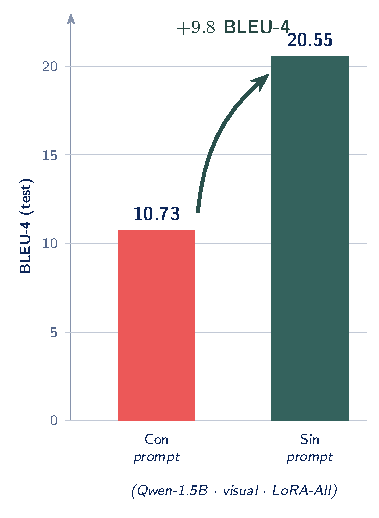
\includegraphics[height=0.66\textheight]{images/experimentacion/prompt_effect}
        \end{center}
        \column{0.5\textwidth}
        \footnotesize
        Con \textit{finetuning}, el modelo se condiciona directamente sobre los
        \textbf{tokens visuales}. El \textit{prompt} textual \alert{compite} con ellos por la
        atención y actúa como ruido.
        \vspace{0.5em}

        Eliminarlo recupera casi \textbf{10 puntos} de BLEU-4 $\rightarrow$ mejor configuración de 1.5B (\textbf{20.55}).
    \end{columns}
\end{frame}

%------------------------------------------------

% --- Slide 9: escalado ---
\begin{frame}{Escalado: el tamaño importa más que la estrategia}
    \begin{center}
        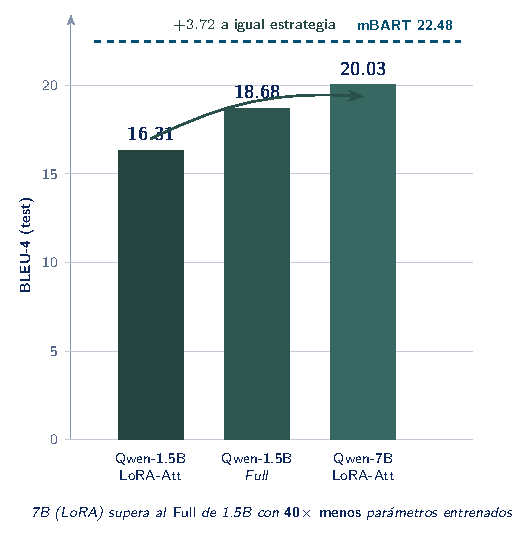
\includegraphics[height=0.64\textheight]{images/experimentacion/scaling_bar}
    \end{center}
    \begin{center}
        \small \textbf{Qwen-7B} con LoRA-Att ($20.03$) supera al \textit{finetuning} completo de
        1.5B ($18.68$): con datos escasos, la \alert{capacidad del modelo base} manda.
    \end{center}
\end{frame}

%------------------------------------------------

% --- Slide 10: comparativa global ---
\begin{frame}{Comparativa global}
    \begin{center}
        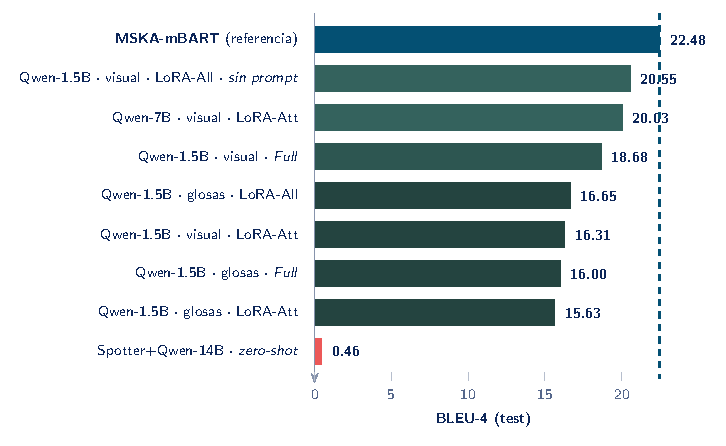
\includegraphics[height=0.82\textheight]{images/experimentacion/results_bar}
    \end{center}
\end{frame}

%------------------------------------------------

% --- Slide 11: coste computacional ---
\begin{frame}{Coste computacional: la relación rendimiento--coste}
    \begin{columns}[c]
        \column{0.62\textwidth}
        \begin{center}
            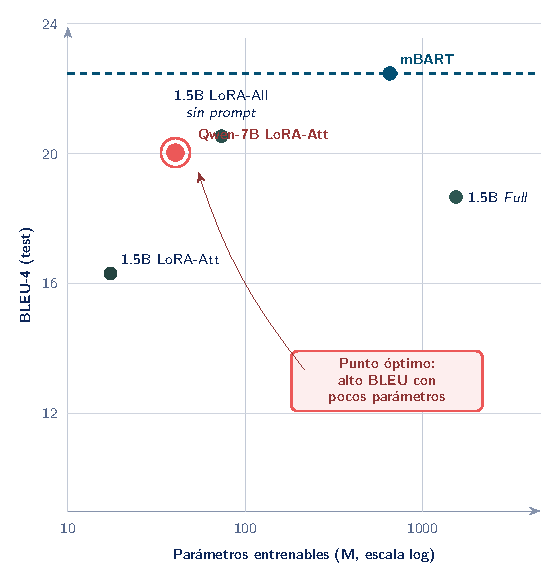
\includegraphics[width=0.75\linewidth]{images/experimentacion/cost_scatter}
        \end{center}
        \column{0.38\textwidth}
        \footnotesize
        mBART entrena \textbf{657\,M} de parámetros; \textbf{Qwen-7B LoRA-Att} solo \textbf{40\,M}.
        \begin{block}{Punto óptimo}
            \footnotesize Con $\sim$2.2$\times$ la memoria de 1.5B, el 7B logra $+3.72$ BLEU-4:
            la mayor ganancia por coste de toda la batería.
        \end{block}
    \end{columns}
\end{frame}

%------------------------------------------------
\section{Conclusiones y trabajo futuro}
%------------------------------------------------



%------------------------------------------------

\begin{frame}{References}
    \footnotesize
    \bibliography{reference.bib}
    \bibliographystyle{apalike}
\end{frame}

%------------------------------------------------

\begin{frame}
    \Huge{\centerline{\textbf{Gracias por su tiempo}}}
\end{frame}

%----------------------------------------------------------------------------------------

\end{document}
